\section{Candidate-Derived Scores on Three Fitted Gaussian Maps}
\label{app:candidatescore}
The preceding scores use reference-derived alternatives. A subsequent gate
instead starts from the Gaussian mean maps already fitted to 8,192-particle
stacks (Appendix~\ref{app:experiments}), with supplied consensus poses. It uses
no external reference map to choose a region or contrast. Each 64-cubed signed
candidate is normalized to unit coefficient norm and interpreted as physical
cells. A 20-\AA\ Gaussian smoothing selects its highest density peak in the
central half-field cube; a same-width Gaussian mask $g$ defines a nominated
regional perturbation. The field sizes come from the saved candidate files.
Full removal changes the candidates' relative $L^2$ norm by .0871, .2655 and
.1464 on 10028, 10049 and 10076 respectively. Smaller deletion amounts scale
these changes linearly. This normalization and the inherited first transfer/
noise profile are a specified simulator, not an experimental SNR calibration.

\subsection{Candidate-only design and its interpretation}
For each candidate, 4,096 independent Haar training views provide mean moment
vectors $\bar\phi_0$ and $\bar\phi_{.25}$ for the candidate and a 25\%
regional deletion. The raw score direction is their normalized difference.
A second direction projects that difference orthogonally to the mean power
and mean bispectrum blocks before normalizing. These blocks have disjoint
coordinates and scale as $a^2$ and $a^3$ under global amplitude, so the
scale-orthogonal contrast's candidate mean is zero for every amplitude on
that finite training law. This identity does not assert exact zero mean
under the continuous viewing law. The threshold is the midpoint between
the training candidate and 25\%-deletion means. Power-only and combined
moments, with both raw and scale-orthogonal directions, give four fixed
scores per candidate. All twelve directions are nonzero.

This is a classical matched contrast with nuisance-mean projection, not a
new learning principle. It avoids an external true-map alternative, but still
assumes a hand-specified local error family. A rejection tests the complete
candidate under the declared image simulator. It cannot uniquely attribute
an error to the nominated region: other structural or imaging errors can
change the same statistic. Non-rejection is not a regional-density confidence
interval. Moment-based structure comparison and independent-particle validation
remain directly relevant prior art \citep{momentmetrics2024,independent2020}.

\subsection{Independent simulations and all-case comparison}
Each stack receives 32,768 fresh calibration views, two groups of 32 noises,
16 amplitude cells and fixed center $b=.5$. Independent testing uses 131,072
Haar views and retains regional deletions $0/.1/.25/.5/1$ at amplitudes
$.9/1/1.1$, with common noise across alternatives and scores. All seven
calibration procedures from Appendix~\ref{app:viewvariance}, five density
caps and three sample sizes are compared separately. The four classical
comparators were declared while calibration was still running, before any
held-out rejection result was computed. No minimum across scores or methods
is used as an aggregate test. The archive contains 1,260 method rows and
18,900 scalar rejection projections.

\begin{figure*}[t]
\centering
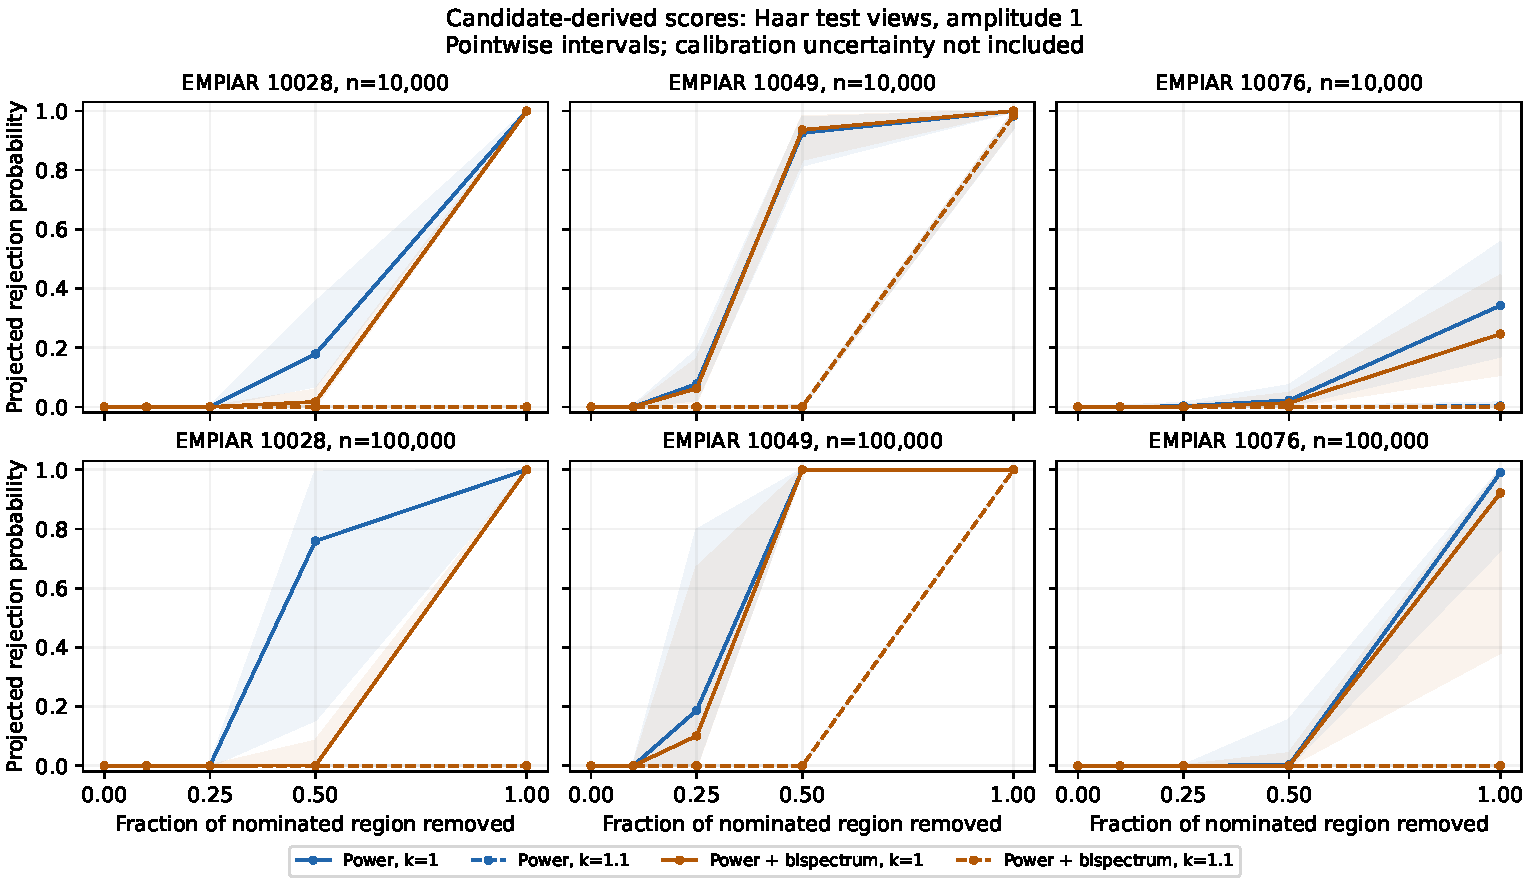
\includegraphics[width=\textwidth]{figures/candidate-score-projections.pdf}
\caption{Candidate-derived local-deletion simulation: scale-orthogonal scores
with the paired viewing-variance procedure, at amplitude one. Lines join the
five tested deletion amounts; shaded bands transform pointwise 95\% intervals
for independent single-image event probabilities. They exclude calibration
variability and are not simultaneous bands or experimentally observed power.
Both raw directions, the other amplitudes and all classical comparators remain
in the complete CSV.}
\label{fig:candidatescore}
\end{figure*}

At $n=10^4$, $\kappa=1$, amplitude one, the paired method's projections for
25\% deletion are .0000225/.000000893 on 10028, .0776/.0625 on 10049,
and .00263/.000846 on 10076 (power/combined). At 50\% deletion they rise
to .178/.0169, .926/.936 and .0224/.0130 respectively. Full deletion is
much easier on the first two candidates; 10076 remains .342/.246 at this
sample size. These results reveal sensitivity limits rather than three-stack
success on small perturbations (Figure~\ref{fig:candidatescore}).

The earlier comparator ordering reverses in some cases. At $\kappa=1.1$,
$n=10^4$, full deletion and amplitude one, the scale-orthogonal power score
on 10028 has projection $4.68\times10^{-7}$ with paired variance, .220
with DKW CVaR, and .426 with split CVaR. On 10049, paired variance gives
.983 and split CVaR .9997; on 10076 they give .00296 and .00113. No
procedure dominates these cases. The paired variance upper bounds for the
three power scores are .02655, .005502 and .001367. Unlike the preceding
selected oracle scores, their raw product estimates are .02558, .005236
and .001302, with nontrivial mean-distance subtraction. The full decomposition
is archived. These data do not support a general superiority claim for the
paired construction, particularly when viewing variation is substantial.

All zero-deletion amplitude controls are retained. At $n=10^4$, the largest
correct-null point projection across methods/scores/caps/amplitudes is .0537.
This single-image Monte Carlo estimate is not an exact false-rejection rate.
Actual testing of 128 disjoint groups of 1,024 images yields at most 7/128
rejections across 1,260 correct-null cells; its pointwise exact 95\% interval
is [.0223,.1094]. Calibration is fixed and cells share draws, so these cells
cannot be pooled as independent replications. The complete archive retains
6,300 group-outcome cells. An unconditional error study over calibration
repetitions remains outstanding.

Independent FFT convolution reproduces all three chosen regions. Separate
feature arithmetic and least-squares projection reproduce all directions within
$7.9\times10^{-15}$. Separable physical sums, 768 first-view calibration
cubics and 180 direct held-out scores are checked; the largest score difference
is $2.5\times10^{-11}$. Every event count, 1,680 minimal critical values,
6,300 group-count vectors and 18,900 rejection projections replay. These
checks do not establish experimental nuisance calibration or global arithmetic
certification. No full-paper acceptance reassessment has occurred.

\section{Covariance-Aware Scores and Simulation Allocation}
\label{app:fisherscore}
The candidate-derived contrast above ignores feature covariance. We therefore
run a fresh classical comparison, preserving the same three candidate maps,
regions, deletion amounts, noise/transfer model and seven calibration methods.
No previously viewed calibration or test draw enters the new experiment.
Each candidate receives 65,536 new Haar training views, with one independent
Gaussian noise per view. Exact conditional feature means determine the null
and 25\%-deletion mean gap $d$, while noisy candidate features determine an
unbiased sample covariance $\widehat\Sigma$. Both feature families compare
a Euclidean matched direction and a constrained Fisher direction, sharing
the same training means. The shrinkage constant is fixed at .1, without tuning:
\[
 S=.9\widehat\Sigma+.1\,\operatorname{tr}(\widehat\Sigma)I/p.
\]
This is classical covariance-aware discriminant design
\citep{friedman1989rda}, not a new learning principle. The alternative
features need not be Gaussian or share the null covariance; $S$ supplies
only a score-design criterion, not the test calibration.

\paragraph{Constrained Rayleigh calculation.}
Let $U$ contain the nonzero, separately normalized null power and bispectrum
mean blocks. These columns have disjoint support. For positive-definite $S$,
define
\[
 r=S^{-1}d-S^{-1}U(U^\top S^{-1}U)^{-1}U^\top S^{-1}d.
\]
The second term is absent when $U$ is empty. Then $U^\top r=0$ and
$Sr=d-Uc$ for some $c$. Thus every feasible $h$ satisfies
$h^\top d=h^\top Sr$, and Cauchy--Schwarz gives
\[
 \frac{(h^\top d)^2}{h^\top Sh}\le r^\top Sr.
\]
Equality holds for nonzero $h$ proportional to $r$; if $r=0$, all feasible
mean gaps vanish. The implemented direction is $r/\|r\|$, with positive
orientation toward the alternative, and the threshold is the training
mean midpoint. The separate block constraints remove global amplitude means
on the finite training law, as above. They do not remove viewing shifts,
variance changes or finite-training error. This elementary optimization
identity does not establish uniformly optimal test power. Independent
calibration permits conditioning on any fixed training result and then
integrating the existing conditional error bound over that training sample.

\subsection{Fresh all-case comparison}
Each stack uses 32,768 new calibration views, two 32-noise groups and 16
amplitude cells, followed by 131,072 independent test views. We retain all
18,900 projections and 6,300 repeated-group cells. To compare Fisher and
matched scores, two 97.5\% exact single-image probability intervals are
transformed by their respective binomial rejection rules. Subtracting
opposite endpoints gives at least 95\% pointwise coverage for the difference,
conditional on training/calibration, by a union bound. This construction
allows dependence between scores. All 9,450 differences and joint event
tables are retained; intervals are not simultaneous across these comparisons.

\begin{figure*}[t]
\centering
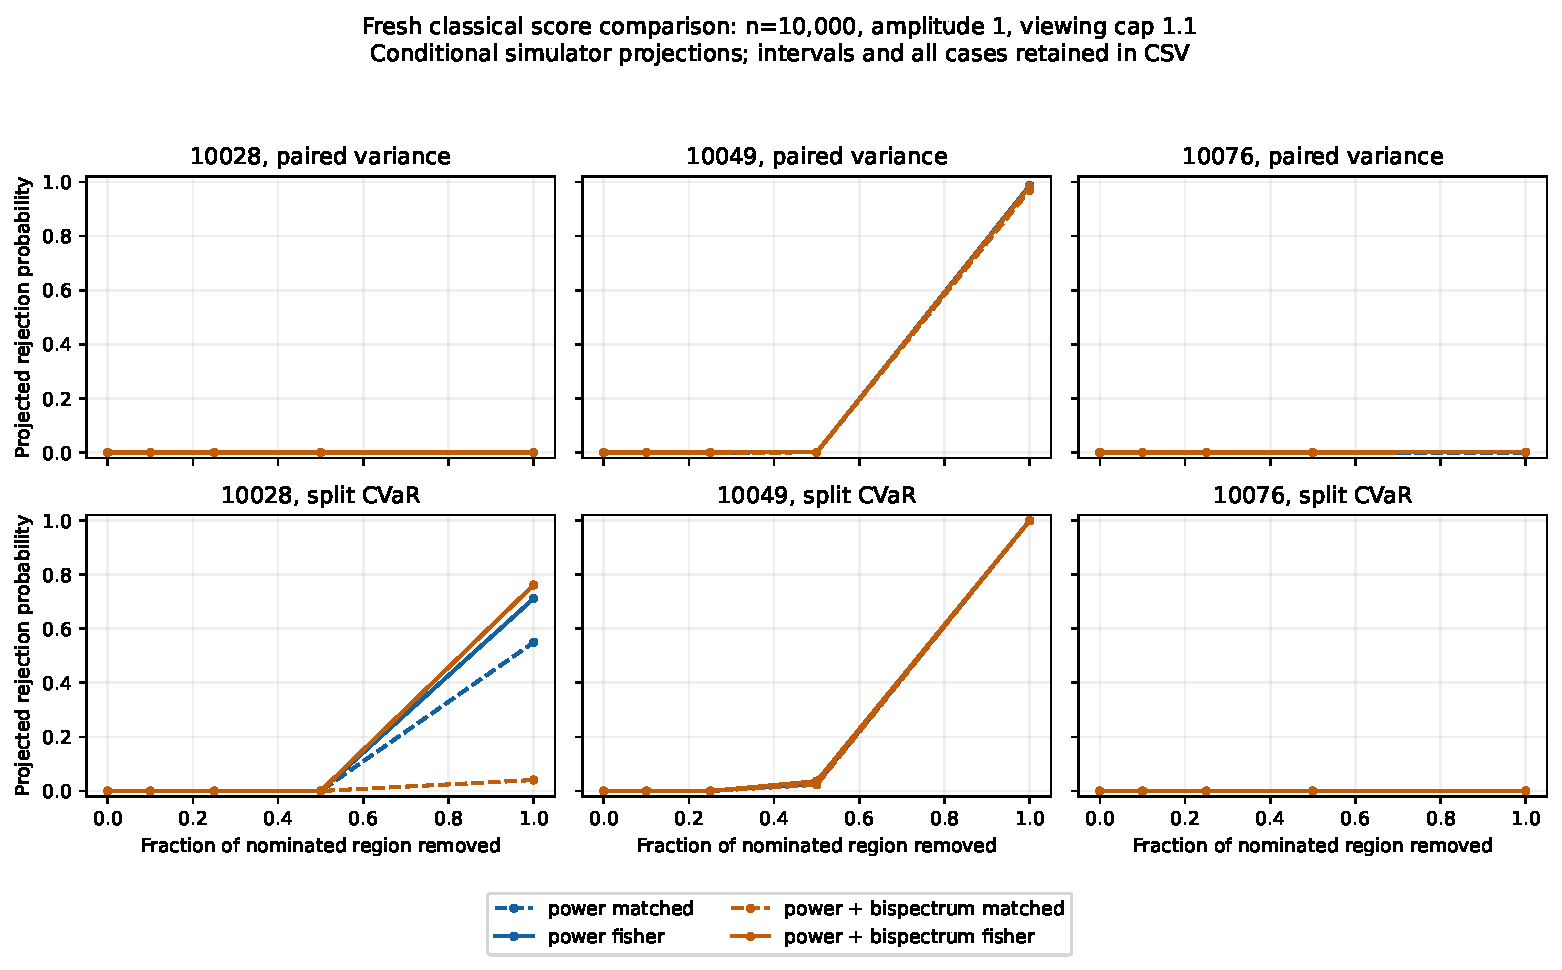
\includegraphics[width=.94\textwidth]{figures/fisher-score-projections.pdf}
\caption{Fresh covariance-aware comparison at $n=10^4$, amplitude one and
viewing cap 1.1. Solid curves use Fisher scores and dashed curves their
matched counterparts. These are conditional simulator projections, with
pointwise individual and difference intervals retained in the complete CSV.
The two calibration procedures are distinct tests; their minimum is not
used as a combined test.}
\label{fig:fisherscore}
\end{figure*}

For 10028, combined-moment training squared separation rises from .00109 to
.00170; its held-out counterpart rises from .00102 to .00161. At $n=10^4$,
$\kappa=1$ and 50\% deletion, paired-variance rejection projections rise
from .0310 to .269 for combined moments and .216 to .345 for power.
With full deletion and $\kappa=1.1$, the combined split-CVaR projection
rises from .0407 to .762; the pointwise difference interval is [.406,.899].
These improvements do not resolve smaller changes:
at 25\% deletion, $\kappa=1$ and $n=10^4$, the Fisher paired projections
are .000156/.0000765 on 10028, .0603/.0513 on 10049, and
.000454/.000259 on 10076 (power/combined). Several 10076 point estimates
are worse under Fisher scoring. Its training criterion is optimal only for
the declared covariance and constraints, and a better mean-to-variance ratio
does not ensure a better robust rejection test.

More particles need not rescue a conservative test whose calibrated probability
bound exceeds the alternative event probability. At $n=10^5$, 25\% deletion
and $\kappa=1$, the 10028 and 10076 projections remain very small. On
10049, the power/paired projection rises from .0420 to .0941, but the
conservative pointwise interval for the difference is $[-.591,.740]$.
This does not resolve improvement at that case. These intervals exclude
calibration variability and are especially wide after the large-$n$
nonlinear transform.

The largest correct-null $n=10^4$ projection is .0000273, with pointwise
interval [.00000236,.000239]. The largest actual correct-null repeated-group
count is 2/128, with exact interval [.00190,.0553]. These are conditional
controls, not 1,260 independent calibration repetitions. Independent replay
reproduces all three full feature covariances within $1.5\times10^{-13}$
and all twelve score directions within $1.4\times10^{-14}$ using a
null-space optimizer. All 420 probability bounds, 1,680 minimal critical
values, 18,900 projections and 6,300 group vectors replay. First-view physical
sums, 768 calibration cubics and all training-noise draws are also checked.
Twenty-five targeted tests pass. Experimental calibration, regional
attribution and useful small-error sensitivity remain unresolved.

\subsection{Equal-noise-budget replica allocation}
The grouped envelope contains a nested maximum of empirical amplitude-cell
means. For two inner sample blocks, convexity gives
\[
 \max_j\frac{x_j+y_j}{2}\le\frac{\max_j x_j+\max_j y_j}{2}.
\]
Thus doubling replicas decreases this envelope in expectation at a fixed view.
It does not ensure a tighter confidence bound when the number of independent
views is reduced. This is a classical nested-simulation issue; antithetic
multilevel methods for maxima and tail risk are relevant prior art
\citep{gilesgoda2018,gileshajiali2019}. Their complexity assumptions and
finite-sample validity do not transfer automatically to our problem.

A frozen follow-up compares the original $(M,L)=(32768,32)$ calibration
with new $(8192,128)$ calibration, using all four fixed scores on each stack.
Both use two groups and 2,097,152 conditional noise draws, with different
Fourier costs and wall times. Both allocations are evaluated on the same
131,072 fresh held-out views per stack, distinct from the preceding study.
Every method, cap, deletion and amplitude is retained: 37,800 scalar
projections and 12,600 actual repeated-group cells. There is no unadjusted
minimum over the two allocations and no claim of optimized allocation.

All twelve estimated grouped means decrease, by about .0028--.0038, but
most joint mean upper bounds on the first two stacks increase. For example,
the 10028 combined Fisher mean decreases from .522783 to .519328 while
its upper bound increases from .527256 to .529238. On the new test draws,
its $n=10^4$, $\kappa=1.1$, full-deletion split-CVaR projection decreases
from .838 to .692. On 10076 the same comparison increases from .000182
to .00796, still weak. At $\kappa=1$ and 25\% deletion, all four 10076
paired-variance projections remain below .00087 under the larger group.
Changes include finite-calibration variation; one calibration per allocation
cannot establish an expected allocation advantage or isolate nested-max bias.

The largest correct-null $n=10^4$ projection is .0000790, with pointwise
interval [.00000779,.000605]. The largest actual null count is 1/128,
with exact interval [.000198,.0428]. Calibration is fixed and cells share
draws. Independent replay verifies the twelve inherited scores, 420 new bounds,
3,360 minimal critical counts, every projection/group vector and 3,072
first-view cubics. Both calibration realizations remain archived.

